\documentclass[10pt,letterpaper]{article}\usepackage[]{graphicx}\usepackage[]{color}
%% maxwidth is the original width if it is less than linewidth
%% otherwise use linewidth (to make sure the graphics do not exceed the margin)
\makeatletter
\def\maxwidth{ %
  \ifdim\Gin@nat@width>\linewidth
    \linewidth
  \else
    \Gin@nat@width
  \fi
}
\makeatother

\definecolor{fgcolor}{rgb}{0.345, 0.345, 0.345}
\newcommand{\hlnum}[1]{\textcolor[rgb]{0.686,0.059,0.569}{#1}}%
\newcommand{\hlstr}[1]{\textcolor[rgb]{0.192,0.494,0.8}{#1}}%
\newcommand{\hlcom}[1]{\textcolor[rgb]{0.678,0.584,0.686}{\textit{#1}}}%
\newcommand{\hlopt}[1]{\textcolor[rgb]{0,0,0}{#1}}%
\newcommand{\hlstd}[1]{\textcolor[rgb]{0.345,0.345,0.345}{#1}}%
\newcommand{\hlkwa}[1]{\textcolor[rgb]{0.161,0.373,0.58}{\textbf{#1}}}%
\newcommand{\hlkwb}[1]{\textcolor[rgb]{0.69,0.353,0.396}{#1}}%
\newcommand{\hlkwc}[1]{\textcolor[rgb]{0.333,0.667,0.333}{#1}}%
\newcommand{\hlkwd}[1]{\textcolor[rgb]{0.737,0.353,0.396}{\textbf{#1}}}%
\let\hlipl\hlkwb

\usepackage{framed}
\makeatletter
\newenvironment{kframe}{%
 \def\at@end@of@kframe{}%
 \ifinner\ifhmode%
  \def\at@end@of@kframe{\end{minipage}}%
  \begin{minipage}{\columnwidth}%
 \fi\fi%
 \def\FrameCommand##1{\hskip\@totalleftmargin \hskip-\fboxsep
 \colorbox{shadecolor}{##1}\hskip-\fboxsep
     % There is no \\@totalrightmargin, so:
     \hskip-\linewidth \hskip-\@totalleftmargin \hskip\columnwidth}%
 \MakeFramed {\advance\hsize-\width
   \@totalleftmargin\z@ \linewidth\hsize
   \@setminipage}}%
 {\par\unskip\endMakeFramed%
 \at@end@of@kframe}
\makeatother

\definecolor{shadecolor}{rgb}{.97, .97, .97}
\definecolor{messagecolor}{rgb}{0, 0, 0}
\definecolor{warningcolor}{rgb}{1, 0, 1}
\definecolor{errorcolor}{rgb}{1, 0, 0}
\newenvironment{knitrout}{}{} % an empty environment to be redefined in TeX

\usepackage{alltt}
\usepackage[top=0.85in,left=1.75in,footskip=0.75in]{geometry}

% amsmath and amssymb packages, useful for mathematical formulas and symbols
\usepackage{amsmath,amssymb}

% Use adjustwidth environment to exceed column width (see example table in text)
\usepackage{changepage}

% Use Unicode characters when possible
\usepackage[utf8x]{inputenc}

% textcomp package and marvosym package for additional characters
\usepackage{textcomp,marvosym}

% cite package, to clean up citations in the main text. Do not remove.
\usepackage{cite}

% Use nameref to cite supporting information files (see Supporting Information section for more info)
\usepackage{nameref,hyperref}

% line numbers
\usepackage[right]{lineno}

% ligatures disabled
\usepackage{microtype}
\DisableLigatures[f]{encoding = *, family = * }

% color can be used to apply background shading to table cells only
\usepackage[table]{xcolor}

% array package and thick rules for tables
\usepackage{array}

% bold math symbols package
\usepackage{bm}

% nice figures and captions
\usepackage{graphicx}

%\usepackage{floatflt}
%\usepackage{nonfloat}
\usepackage{float}
\usepackage{wrapfig}

%\renewcommand{\arraystretch}{1.2}
%\setlength{\tabcolsep}{12pt}

% create "+" rule type for thick vertical lines
\newcolumntype{+}{!{\vrule width 2pt}}

% create \thickcline for thick horizontal lines of variable length
\newlength\savedwidth
\newcommand\thickcline[1]{%
  \noalign{\global\savedwidth\arrayrulewidth\global\arrayrulewidth 2pt}%
  \cline{#1}%
  \noalign{\vskip\arrayrulewidth}%
  \noalign{\global\arrayrulewidth\savedwidth}%
}

% \thickhline command for thick horizontal lines that span the table
\newcommand\thickhline{\noalign{\global\savedwidth\arrayrulewidth\global\arrayrulewidth 2pt}%
\hline
\noalign{\global\arrayrulewidth\savedwidth}}


% Remove comment for double spacing
%\usepackage{setspace} 
%\doublespacing

% Text layout
\raggedright
\setlength{\parindent}{0.5cm}
\textwidth 5.25in 
\textheight 8.75in

% Bold the 'Figure #' in the caption and separate it from the title/caption with a period
% Captions will be left justified
\usepackage[aboveskip=1pt,labelfont=bf,labelsep=period,justification=raggedright,singlelinecheck=off]{caption}
\renewcommand{\figurename}{Fig}

% Use the PLoS provided BiBTeX style
%\bibliographystyle{plos2015}


% Remove brackets from numbering in List of References
\makeatletter
\renewcommand{\@biblabel}[1]{\quad#1.}
\makeatother



% Header and Footer with logo
\usepackage{lastpage,fancyhdr,graphicx}
\usepackage{epstopdf}
%\pagestyle{myheadings}
\pagestyle{fancy}
\fancyhf{}
%\setlength{\headheight}{27.023pt}
%\lhead{\includegraphics[width=2.0in]{PLOS-submission.eps}}
\rfoot{\thepage/\pageref{LastPage}}
\renewcommand{\headrulewidth}{0pt}
\renewcommand{\footrule}{\hrule height 2pt \vspace{2mm}}
\fancyheadoffset[L]{2.25in}
\fancyfootoffset[L]{2.25in}
\lfoot{\today}


\restylefloat{figure}


%% Include all macros below

\newcommand{\lorem}{{\bf LOREM}}
\newcommand{\ipsum}{{\bf IPSUM}}

\def\lf{\left\lfloor}   
\def\rf{\right\rfloor}

\def\ri{R_i}
\def\rj{R_j}
\def\kmi{k_{M_i}}
\def\khi{k_{H_i}}
\def\hji{H_{j_i}}
\def\ma{\overline{M}_a}
\def\ha{\overline{H}_a}
\def\mnu{M_\nu}
\def\hnu{H_\nu}
\def\myd{\text{diff}}
\def\ka{\bar{k}_\alpha}
\def\mji{M_{j_i}}

%% END MACROS SECTION
\IfFileExists{upquote.sty}{\usepackage{upquote}}{}
\begin{document}
\vspace*{0.2in}

% Title must be 250 characters or less.
% \begin{flushleft}
{\Large
\textbf\newline{Blessings of Dimensionality: Theoretical analysis of nearest-neighbor projected-distance methods for detecting interactions in high dimension} % Please use "sentence case" for title and headings (capitalize only the first word in a title (or heading), the first word in a subtitle (or subheading), and any proper nouns).
}
%\newline
% Insert author names, affiliations and corresponding author email (do not include titles, positions, or degrees).
\begin{center}
  \begin{tabular}{l}
  Bryan A. Dawkins$^{\text{1}}$, Trang T. Le$^{\text{2}}$ and Brett A. McKinney$^{\text{1,3,}*}$ \\
  $^{\text{1}}$Department of Mathematics, University of Tulsa, Tulsa, OK 74104, USA \\
  $^{\text{2}}$Department of Biostatistics, Epidemiology and Informatics, University of \\
  \hphantom{2}Pennsylvania, Philadelphia, PA 19104 \\
  $^{\text{3}}$Tandy School of Computer Science, University of Tulsa, Tulsa, OK 74104, USA.
  \end{tabular}
\end{center}


% \end{flushleft}
% Please keep the abstract below 300 words
\section*{Abstract}
It is commonly known that high-throughput data has many inherent statistical challenges, such as multiple testing, sparsity and over fitting. Collectively these challenges are known as the Curse of Dimensionality. Here we highlight an important Blessing of Dimensionality: the ability to identify interactions with nearest neighborhoods. We review nearest-neighbor concepts for finding interactions, and we derive important distribution moments for distance metrics in high dimensional spaces. We use these theoretical results and simulated data to offer recommendations for computational approaches to find nearest neighbors in high dimension. We discuss ways to maximize the blessings and minimize the curses of dimensionality to reliably identify interactions.  

\section*{Author summary}

\linenumbers

\section*{Introduction}

Relief-based methods identify interacting attributes as important by using nearest-neighbor information in higher dimensions (the ``blessings of dimensionality'' ). Myopic methods, such as univariate tests, that do not account for information from higher dimensions, are susceptible to false negatives when there are interactions. For example in the plot of variable A versus C in a three-variable simulation (Fig.~\ref{fig:2dAvC}a), variable A appears to show no difference between cases and controls (the marginal group means are the same). However, A is actually simulated to have a strong differential correlation with B, conditioned on the outcome variable (Fig.~\ref{fig:2dAvB}b). Current Relief-based methods determine the importance of an attribute by computing the average difference of a target instance (X) and its nearest instance form the same class (Hit) projected onto the attribute A dimension ($d_{\text{X,H}}(A)$) subtracted from the projected difference of target X and its nearest instance from the opposite class (Miss) ($d_{\text{X,M}}(A)$). When the inequality $d_{\text{X,M}}(A)>d_{\text{X,H}}(A)$, it suggests that attribute A is useful for discriminating between cases and controls.  

%\begin{figure}[h!]
%%\begin{center}
%\begin{minipage}[c]{0.4\textheight}
%\centering
%		\framebox{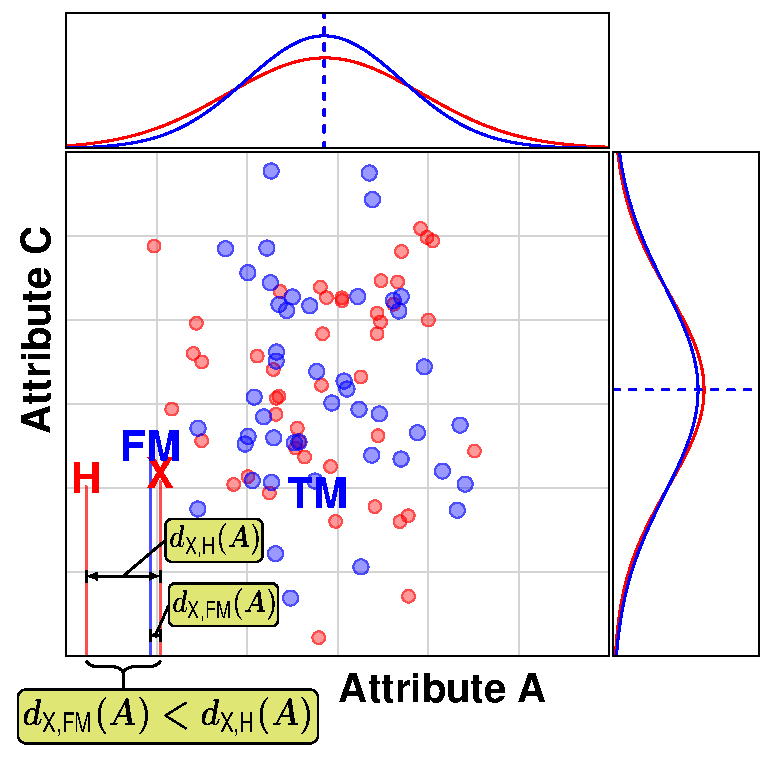
\includegraphics[width=0.8\textwidth]{glmSTIR_figure_2D_final_CvsA.pdf}}
%\end{minipage} \hspace{-0.4cm}
%\begin{minipage}[c]{0.5\textwidth}
%\centering
%\caption{{\bf Imposters vs true neighbors in the presence of interactions with three variables}. Scatter plot of simulated irrelevant Attribute C with a functional Attribute A {\bf(a)}. None of the attributes has a main effect, but Attribute B and C interact through differential correlation {\bf(b)}. Computing nearest neighbors with irrelevant attributes {\bf(a)} or lower dimensions leads to imposter nearest neighbors and degrades the ability of Relief-based methods to identify interaction effects. Computing distances in only these two dimensions leads to an imposter false miss (FM) for the nearest neighbor from the opposite outcome class for target instance X. This imposter leads to attribute A predicting closer projected distances for misses than hits (H), which incorrectly indicates that A is a poor discriminator (yellow boxes in {\bf a}). Computing nearest neighbors in higher dimensions {\bf(c-d)} or with the correct interaction partner leads to imposter nearest neighbor (FM) being replaced by the true nearest miss neighbor (TM) for target instance X, which correctly leads to attribute A predicting closer projected distances for hits (H) than misses, which is an indication that attribute A is a good discriminator (yellow boxes {\bf(b)}).}\label{fig:2dAvC}
%\end{minipage}
%%\end{center}
%\end{figure}

\newpage

\begin{figure}[ht!]
\begin{wrapfigure}{l}{0.6\textwidth}
    \vspace{-12pt}
	\centering
	\framebox{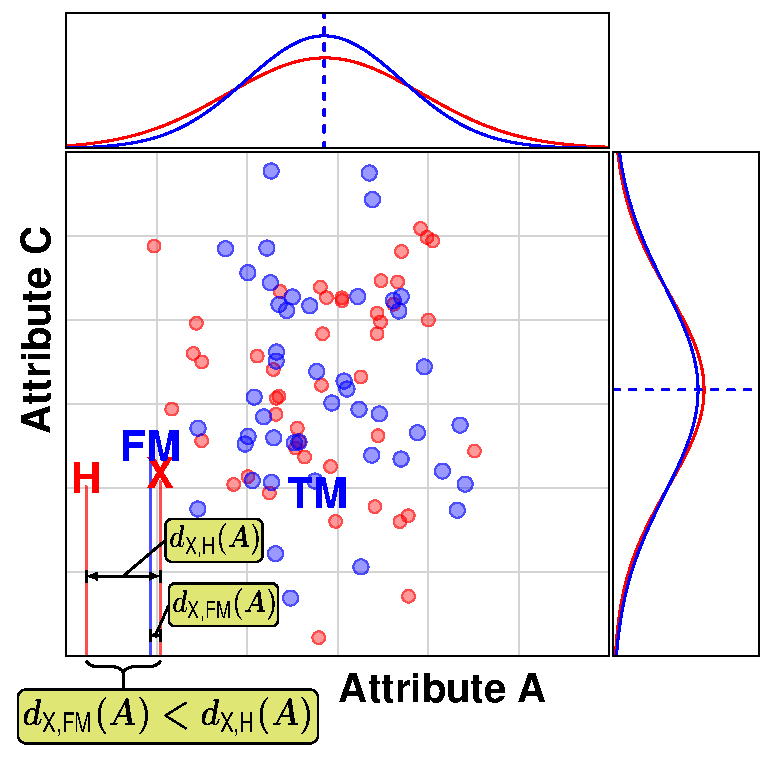
\includegraphics[width=0.55\textwidth]{glmSTIR_figure_2D_final_CvsA.pdf}}
\end{wrapfigure}
\noindent\refstepcounter{figure}\textbf{Fig \thefigure \label{fig:2dAvC}.} \textbf{Imposters vs true neighbors in the presence of interactions with three variables}. Scatter plot of simulated irrelevant Attribute C with a functional Attribute A \textbf{(a)}. None of the attributes has a main effect, but Attribute B and C interact through differential correlation \textbf{(b)}. Computing nearest neighbors with irrelevant attributes \textbf{(a)} or lower dimensions leads to imposter nearest neighbors and degrades the ability of Relief-based methods to identify interaction effects. Computing distances in only these two dimensions leads to an imposter false miss (FM) for the nearest neighbor from the opposite outcome class for target instance X. This imposter leads to attribute A predicting closer projected distances for misses than hits (H), which incorrectly indicates that A is a poor discriminator (yellow boxes in \textbf{(a)}). Computing nearest neighbors in higher dimensions \textbf{(c-d)} or with the correct interaction partner leads to imposter nearest neighbor (FM) being replaced by the true nearest miss neighbor (TM) for target instance X, which correctly leads to attribute A predicting closer projected distances for hits (H) than misses, which is an indication that attribute A is a good discriminator (yellow boxes \textbf{(b)}).
\end{figure}

Relief-based methods use information from all attributes available to it (omnigenic) to estimate an attribute's importance. However, if relevant higher-dimensional information is not used, even Relief-based methods will miss the effect of A because ``imposter'' neighbors will be used in the attribute estimate (False Miss (FM) in Fig.~\ref{fig:2dAvC}, where $d_{\text{X,FM}}(A)<d_{\text{X,H}}(A)$).  If one were to compute nearest neighbors in the A-C plane (ignoring the B dimension), the nearest miss would be an imposter (FM), which leads to a negative contribution to the importance score for A. One might call this C attribute a type-I confounding attribute because it increases the chances of interacting attributes to be false negatives. When nearest neighbors are calculated based on higher dimensions with relevant information (Fig.~\ref{fig:2dAvB}c), it is clear that TM is closer to X than FM. The imposter (FM) is replaced by the true nearest miss (TM) and attribute A correctly shows a greater projected difference between misses than hits (Fig.~\ref{fig:2dAvB}d $d_{\text{X,TM}}(A)>d_{\text{X,H}}(A)$), which is the signature of an important attribute. Univariate methods still cannot find the importance of A unless the interaction is explicitly modeled, but as long as functional variables A and B are in the space for nearest neighbor calculations (Fig.~\ref{fig:2dAvB}c-d), imposters can be excluded and Relief-based methods will find that A (and B) are important discriminators. 


[Ideas: Relating the increasing $k$ and myopic view to other distance-related method such as MDS/t-SNE vs PCA - local vs global distance - capturing non-linear manifold structure. \url{https://www.kdnuggets.com/2018/08/introduction-t-sne-python.html}]


\begin{figure}[ht!]
%%\begin{center}
\begin{minipage}[c]{0.4\textheight}
\centering 
		\framebox{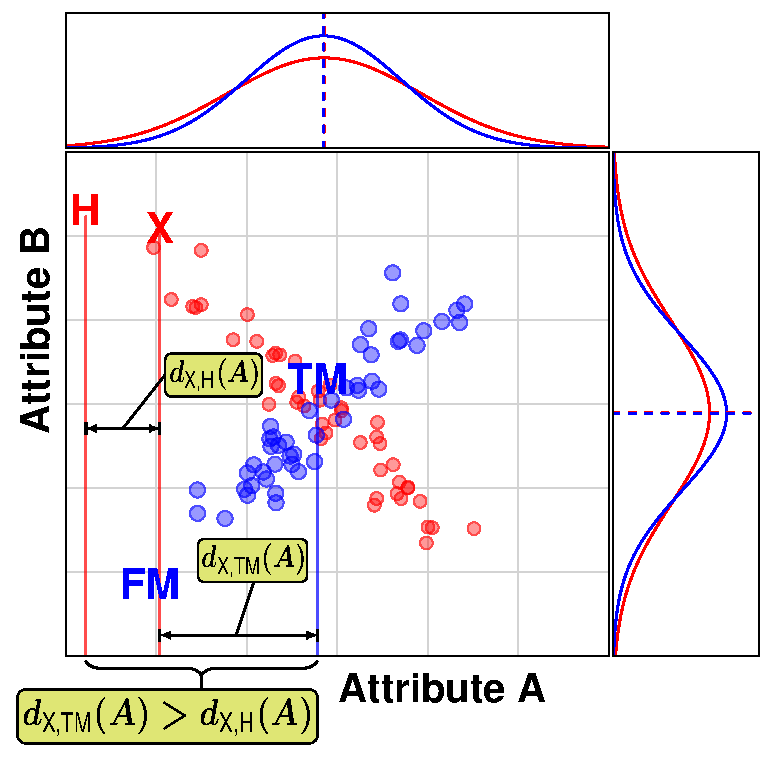
\includegraphics[width=0.8\textwidth]{glmSTIR_figure_2D_final_BvsA.pdf}}
\end{minipage} \hspace{-0.4cm}
\begin{minipage}[c]{0.5\textwidth}
\centering
\caption{{\bf True neighbors}}\label{fig:2dAvB}
\end{minipage}
%%\end{center}
\end{figure}  

\begin{figure}[ht!]
%%\begin{center}
\begin{minipage}[c]{0.4\textheight}
\centering
		\framebox{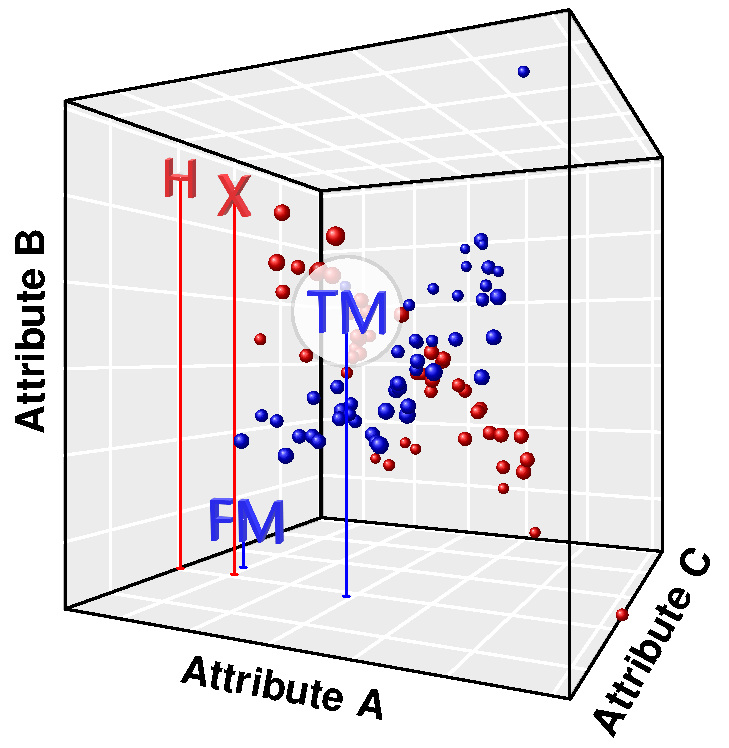
\includegraphics[width=0.8\textwidth]{nice_box_2D_points.pdf}}
\end{minipage} \hspace{-0.4cm}
\begin{minipage}[c]{0.5\textwidth}
\centering
\caption{{\bf 3D AB view}. Still working on this. }\label{fig:3d_c}
\end{minipage}
%%\end{center}
\end{figure}  

\begin{figure}[ht!]
%%\begin{center}
\begin{minipage}[c]{0.4\textheight}
\centering
		\framebox{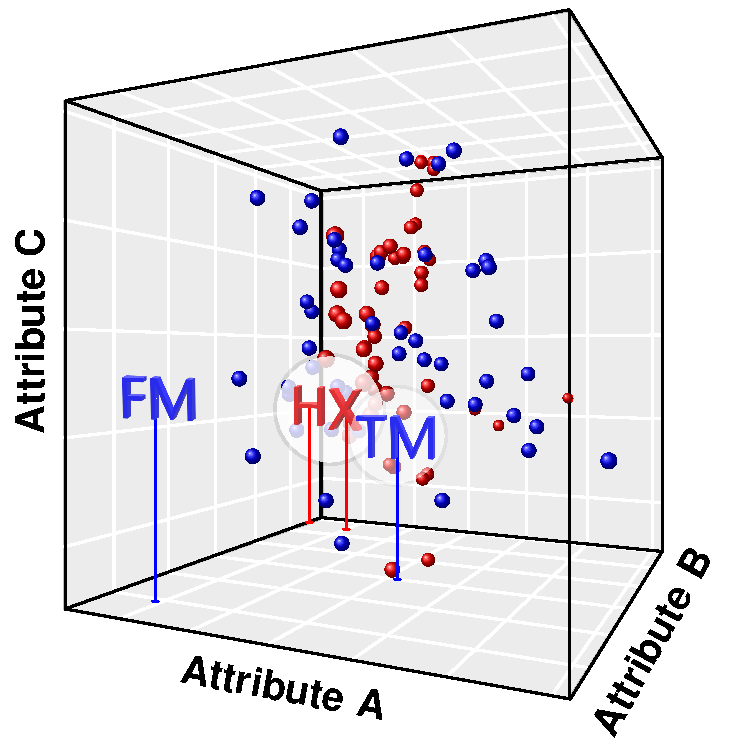
\includegraphics[width=0.8\textwidth]{nice_box_2D_points2.pdf}}
\end{minipage} \hspace{-0.4cm}
\begin{minipage}[c]{0.5\textwidth}
\centering
\caption{{\bf 3D AC view}. Still working on this. }\label{fig:3d_d}
\end{minipage}
%%\end{center}
\end{figure}  
Using same interaction, increase background noise genes to see degrading of A and B Relief importance because of curse of dimensionality (sparseness). 

\section{Neighborhood methods}
NPD methods rely on a neighborhood algorithm for feature selection. One may specify a fixed-k number of neighbors, an average radius SURF, a multiSURF radius that adapts for each instance ~\cite{urbanowicz17}, or a gene-wise adaptive-$k$. 

\section{Derivation of expected k for multiSURF neighborhoods}
The multiSURF radius for an instance is the mean of its distances to all other instances subtracted by $\alpha=1/2$ of the standard deviation of this mean. Previously we showed empirically for balanced case-control datasets that a good constant-$k$ approximation to the expected number of neighbors within the multiSURF radii is $k=m/6$~\cite{stir}, where $m$ is the number of samples. Here we derive a more exact theoretical mean that shows the mathematical connection between neighbor-finding methods. This fixed-$k$ approximation to multi-SURF is independent of the type of data and the particular radii of each instance in the data.
%

The distance between instances $i$ and $j$ in the data set $X^{m \times p}$ of $m$ instances and $p$ attributes is calculated in the space of all attributes ($a \in A$, $|A|=p$) using a metric such as
\begin{equation}\label{eq:D}
% D^{(q)}_{ij}=\left(\sum_{a\in A}|\text{d}^{\text{type}}_{ij}(a)|^q\right)^{1/q},
D^{(q)}_{ij}=\left(\sum_{a\in A}|\text{d}_{ij}(a)|^q\right)^{1/q},
\end{equation}
which is typically Manhattan ($q=1$) but may also be Euclidean ($q=2$). The quantity 
% $\text{d}^{\text{type}}_{ij}(a)$, 
$\text{d}_{ij}(a)$,
known as a ``$\text{diff}$'' in Relief literature, is the projection of the distance between instances $i$ and $j$ onto the attribute $a$ dimension. The 
% ``type'' refers to the data type of the attribute
function $\text{d}_{ij}(a)$ supports any type of attributes
(e.g., numeric continuous versus categorical).
For example, the projected difference between two instances $i$ and $j$ for a continuous numeric ($\text{d}^{\text{num}}$) attribute $a$ may be
%\begin{equation}\label{eq:diff}
%\text{diff}^{(\text{num})}(a,(\ri,\rj))=\frac{|\text{value}(a,\ri)-\text{value}(a,\rj)%|}{\max(a)-\min(a)}.
%\end{equation}
\begin{equation}\label{eq:diff}
\begin{aligned}
\text{d}^{\text{num}}_{ij}(a)&=\text{diff}(a,(i,j))\\
                                            & = {|\hat{X}_{ia}-\hat{X}_{ja}|},
\end{aligned}
\end{equation}
where $\hat{X}$ represents the standardized data matrix $X$.
We use a simplified d$_{ij}(a)$ notation in place of the $\text{diff}(a,(i,j))$ notation that is customary in Relief-based methods.
We omit the division by $\max(a)-\min(a)$ used by Relief to constrain scores to the interval from $-1$ to $1$.
As we show in subsequent sections, NPDR scores are [standardized] regression coefficients with corresponding P values, so any scaling operation at this stage is unnecessary for comparing attribute scores. 
%\emph{Omit: The scaling may alleviate bias in the distance calculation. However, standardizing the data matrix $X$ ($\hat{X}$) should have the same effect without division by $\max(a)-\min(a)$, which has usual distribution properties for distances (expand).}
The numeric d$^{\text{num}}_{ij}(a)$ projection is simply the absolute difference between row elements $i$ and $j$ of the data matrix $X^{m \times p}$ for the attribute column $a$. 

We define the NPDR neighborhood set $\mathcal{N}$ of ordered pair indices as follows. Instance $i$ is a point in $p$ dimensions, and we designate the topological neighborhood of $i$ as $N_{i}$. This neighborhood is a set of other instances trained on the data $X^{m \times p}$ and depends on the type of Relief neighborhood method (e.g., fixed-$k$ or adaptive radius) and the type of metric (e.g., Manhattan or Euclidean). If instance $j$ is in the neighborhood of $i$ ($j \in N_{i}$), then the ordered pair $(i,j) \in \mathcal{N}$ for the projected-distance regression analysis. The ordered pairs constituting the neighborhood can then be represented as nested sets:
\begin{equation}\label{eq:N}
\mathcal{N}=\{\{(i, j)\}_{i=1}^{m}\}_{\{j \ne i : j \in N_{i}\}}.
\end{equation}
The cardinality of the set $\{j \ne i : j \in N_{i}\}$ is $k_i$, the number of nearest neighbors for subject $i$. 

\subsection{Distribution of pairwise distances}
%Discuss Central Limit Theorem argument for the distribution being Gaussian. We can always say this is an assumption, but I think we can invoke the CLT. [I would be cautious here - TTL. We will be cautious invoking the CLT - BAM.]

Suppose that $X_{ia}, X_{ja} \overset{iid}{\sim} \mathcal{F}_X(\mu_X,\sigma^2_X)$ for two fixed and distinct instances $(i,j) \in \mathcal{N}$ and a fixed attribute $a \in \mathcal{A}$. 

It is clear that the magnitude difference, or numeric diff given by Eq. \ref{eq:diff}, between $X_{ia}$ and $X_{ja}$ is another random variable $Z_a$. That is,

\begin{equation}\label{eq:diffDistr}
Z_a = d_{ij}(a) = |X_{ia} - X_{ja}| \sim \mathcal{F}_Z(\mu_z,\sigma^2_z).
\end{equation}

Furthermore, the collection of all magnitude differences between fixed instances $i$ and $j$ is a random sample of size $p$ from $\mathcal{F}_Z(\mu_z,\sigma^2_z)$. That is, $Z_{a_1},Z_{a_2},\dots,Z_{a_p} \overset{iid}{\sim} \mathcal{F}_Z(\mu_z,\sigma^2_Z)$ such that

\begin{equation}\label{eq:AlldiffDistr}
Z_{a_k} = d_{ij}(a_k) = |X_{ia_k} - X_{ja_k}|.
\end{equation}

Therefore, the sum of all $Z_{a_k}$ for $k=1,2,\dots,p$ is asymptotically normal by the Classical Central Limit Theorem (CCLT). Explicitly, this means that

\begin{equation}\label{eq:manhattanAsympt}
D^{(1)}_{ij} = \displaystyle \sum_{k=1}^{p}|X_{ia_k} - X_{ja_k}| = \displaystyle \sum_{k=1}^{p}d_{ij}(a_k) = \displaystyle \sum_{k=1}^{p}Z_{a_k} \overset{.}{\sim} \mathcal{N}(\mu_zp,\sigma^2_zp).
\end{equation}

Therefore, the standard manhattan distance between two distinct and fixed instances $i$ and $j$ is asymptotically normal.

It is also apparent that the squared difference, or squared numeric diff, between $X_{ia}$ and $X_{ja}$ is another random variable $Z^2_{a}$. That is,

\begin{equation}\label{eq:SqudiffDistr}
Z^2_a = d^2_{ij}(a) = (X_{ia} - X_{ja})^2 \sim \mathcal{F}_{Z^2}(\mu_{z^2},\sigma^2_{z^2}).
\end{equation}

Furthermore, the collection of all squared differences between fixed instances $i$ and $j$ is a random sample of size $p$ from $\mathcal{F}_{Z^2}(\mu_{z^2},\sigma^2_{z^2})$. That is, $Z^2_{a_1},Z^2_{a_2},\dots,Z^2_{a_p} \overset{iid}{\sim} \mathcal{F}_{Z^2}(\mu_{z^2},\sigma^2_{z^2})$ such that

\begin{equation}\label{eq:AllSqudiffDistr}
Z^2_{a_k} = (X_{ia_k} - X_{ja_k})^2.
\end{equation}

Therefore, the sum of all $Z^2_{a_k}$ for $k=1,2,\dots,p$ is asymptotically normal by the Classical Central Limit Theorem. Explicitly, this means that

\begin{equation}\label{eq:SquEuclideanAsympt}
\left(D^{(2)}_{ij}\right)^2 = \displaystyle \sum_{k=1}^{p}(X_{ia_k} - X_{ja_k})^2 = \displaystyle \sum_{k=1}^{p}d^2_{ij}(a_k) = \displaystyle \sum_{k=1}^{p}Z^2_{a_k} \overset{.}{\sim} \mathcal{N}(\mu_{z^2}p,\sigma^2_{z^2}p).
\end{equation}

Consider the smooth functional transformation $g(\alpha) = \sqrt{\alpha}$ applied to the random variable given by Eq. \ref{eq:SquEuclideanAsympt}. The Delta Method \cite{allStats} can be applied to show that

\begin{equation}\label{eq:DeltaMethod}
g\left(\left(D^{(2)}_{ij}\right)^2\right) = g\left(\displaystyle \sum_{k=1}^{p}Z^2_{a_k}\right) = \sqrt{\displaystyle \sum_{k=1}^{p} (X_{ia_k} - X_{ja_k})^2} \overset{.}{\sim} \mathcal{N}\left(g(\mu_{z^2}p),[g\prime(\mu_{z^2}p)]^2\sigma^2_{z^2}\right)
\end{equation}

Therefore, the standard Euclidean distance between two fixed and distinct instances $i$ and $j$ is asymptotically normal.

We have considered the distance metric given by Eq. \ref{eq:D} for $q=1$ (Manhattan) and $q=2$ (Euclidean). Without loss of generality, the argument presented previously for $q=2$ can be used to show asymptotic normality of $D^{(q)}_{ij}$ with $q>2$. Therefore, the pairwise distance distribution of $D^{(q)}_{ij}$ is asymptotically normal with the assumption of independently and identically distributed instances. This result is true for any null data distribution, whether continuous or discrete. One can readily verify the normality of distances between independent instances through sampling from any data distribution and plotting the histogram of pairwise distances. Histograms for the case of standard normal data and Manhattan and Euclidean metrics are shown in Figs. \ref{fig:manhattanConverge} and \ref{fig:euclideanConverge}, respectively. For these simulated distances, we fixed $m=100$ and varied $p$ from 10 to 10000. For even a rather small number of predictors, as in the case of $p=10$, the sample distances are approximately normal. As $p$ increases, the normality becomes stronger.

\begin{figure}[ht!]
\centering
		\framebox{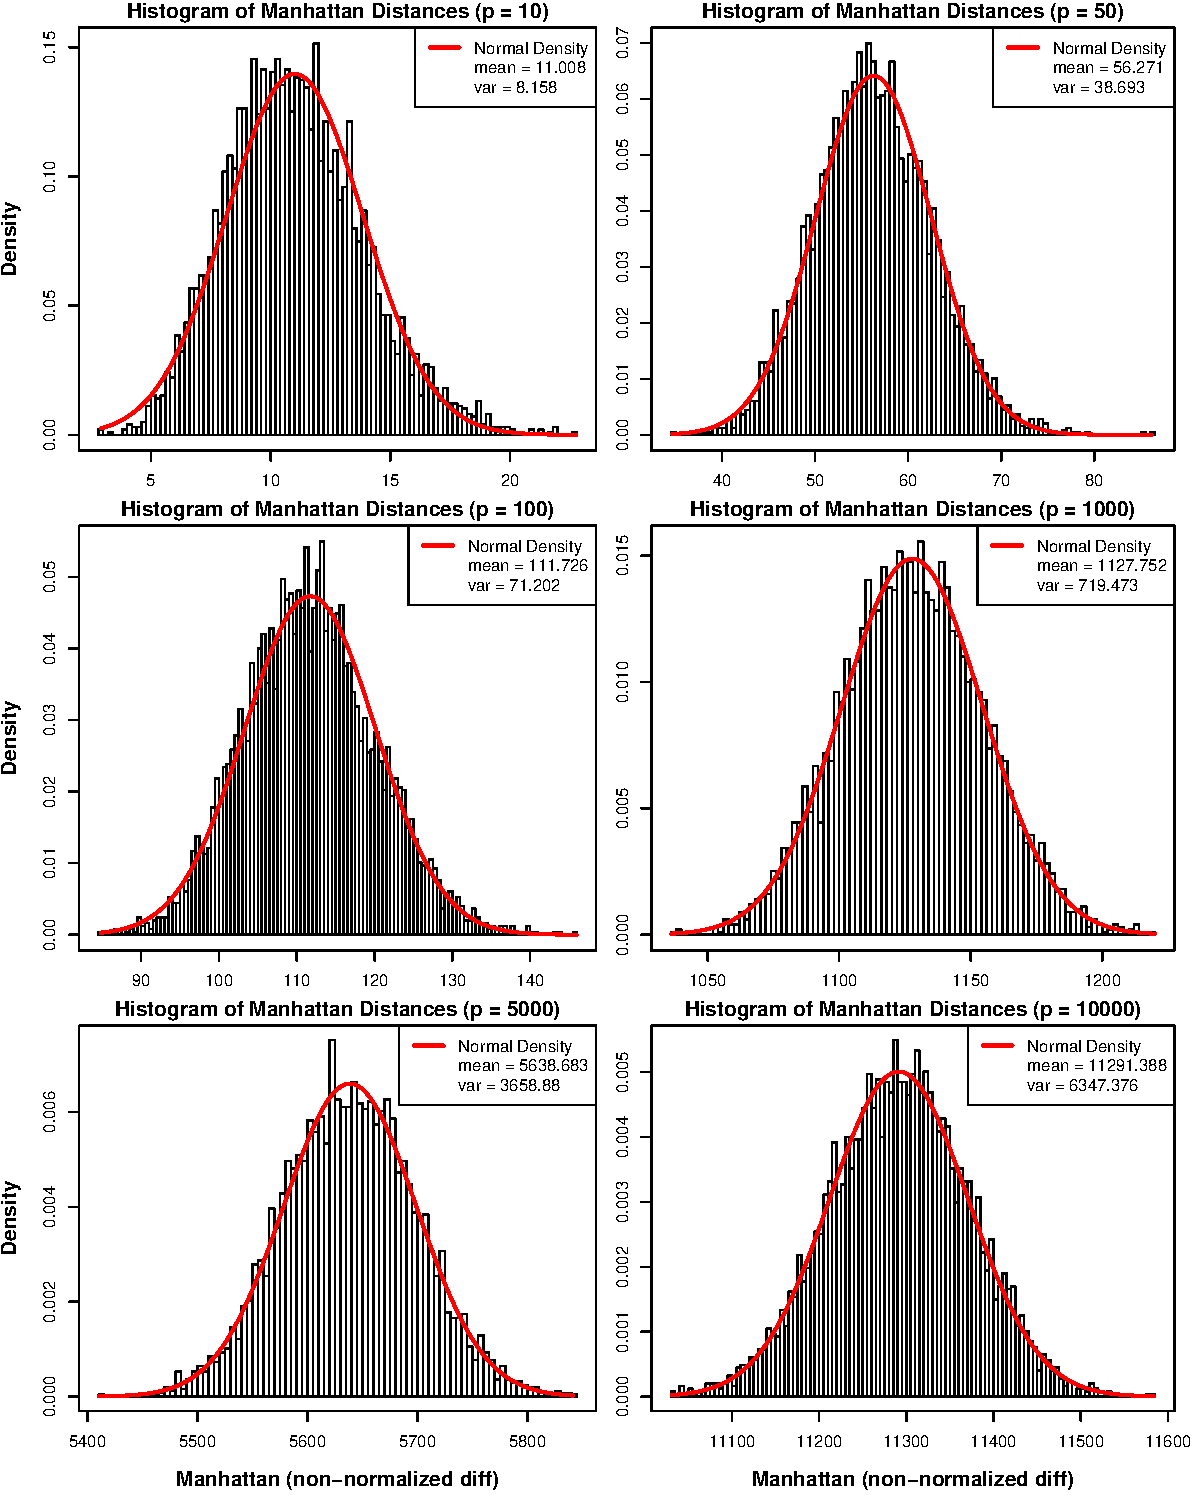
\includegraphics[width=0.95\textwidth]{central_limit_distances-Manhattan-Normal-diffstar.pdf}}
		\caption{Convergence to normality of Manhattan distances between iid random normal instances. For each simulated distance distribution, we fixed $m=100$ instances but varied $p$ from 10 to 10000. It is clear that convergence is rapid, and approximate normality can be safely assumed for even $p=10$.}\label{fig:manhattanConverge}
\end{figure} 

\begin{figure}[ht!]
\centering
		\framebox{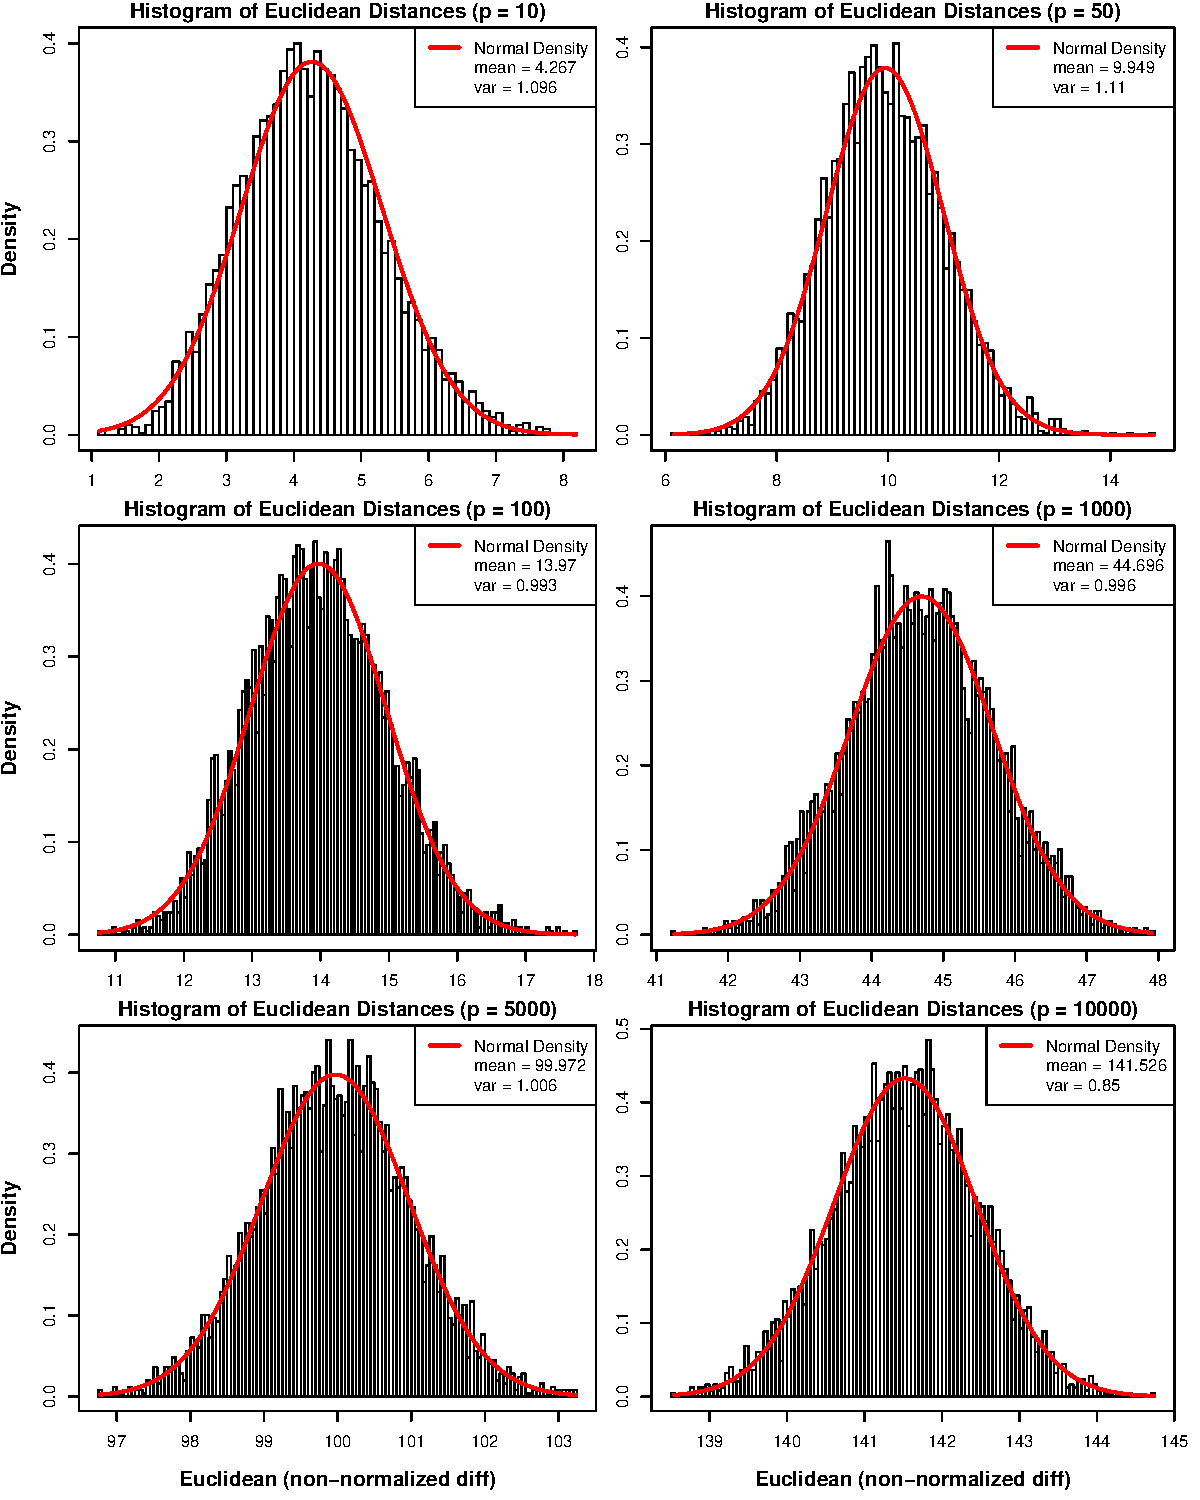
\includegraphics[width=0.95\textwidth]{central_limit_distances-Euclidean-Normal-diffstar.pdf}}
		\caption{Convergence to normality of Euclidean distances between iid random normal instances. For each simulated distance distribution, we fixed $m=100$ instances but varied $p$ from 10 to 10000. It is clear that convergence is rapid, and approximate normality can be safely assumed for even $p=10$.}\label{fig:euclideanConverge}
\end{figure}

For distance based learning methods, all pairwise distances are used to determine relative importances for attributes. The collection of all distances above the diagonal in an $m \times m$ distance matrix does not satisfy the independence assumption used in the previous derivations. This is because of the redundancy that is inherent to the distance matrix calcuation. However, this collection is still asymptotically normal with mean and variance approximately equal to those given in Eqs. \ref{eq:manhattanAsympt} or \ref{eq:DeltaMethod}. Hence, all fixed-radius methods will use a fixed radius that is some fraction of the expected pairwise distance for a given metric and data type. This implies that the probability of a fixed instance $j$ being within a fixed radius of a given instance $i$ can be parameterized by the expected pairwise distance and the variance of the pairwise distance. This probability is obtained by evaluating the normal cumulative distribution function (CDF), with corresponding mean and variance, at the quantile given by some function of the fixed radius. Therefore, we can derive the expected number of neighbors in the neighborhood of a fixed instance $i$. In other words, for sufficiently large data sets, the sample mean of the number of neighbors in a given neighborhood is well approximated by the product between the total number of possible neighbors and the expected probability of an instance being in a given neighborhood. The total number of possible neighbors for a fixed instance $i$ is always $m-1$, but this becomes approximately $\lfloor{\frac{m - 1}{2}}\rfloor$ when delineating between possible hits and misses for balanced data.

\subsection{Predicted number of neighbors in the multiSURF alpha neighborhood}

Regardless of the predictor data type (numeric or categorical), the distribution of the $p$ predictors (uniform, Gaussian, or binomial), or the metric used to compute distances (Manhattan or Euclidean), the $m(m-1)/2$ pairwise distances in the $p$-dimensional space are well approximated by a normal distribution. An instance $j$ is in the adaptive $\alpha$-radius neighborhood of $i$ ($j \in N^{\alpha}_{i}$) under the condition
%\begin{equation}
%\bar{D = \frac{2p}{\sqrt{\pi}}
%\end{equation}
%
%\begin{equation}
%\sigma_{D} = \frac{2p(\pi-2)}{\pi}
%\end{equation}
%
\begin{equation}
D_{ij} \le \, R_i^{\alpha} \implies j \in N^{\alpha}_{i},
\end{equation}
where the threshold radius for instance $i$ is
\begin{equation}
R_i^{\alpha} =  \bar{D}_i - \alpha \, \sigma_{\bar{D}_i}
\end{equation}
and
\begin{equation}
\bar{D}_i = \frac{1}{m-1} \sum_{j \ne i} D^{(\cdot)}_{ij}
\end{equation}
is the average of instance $i$'s pairwise distances (using Eq. D Equation) with standard deviation $\sigma_{\bar{D}_i}$. MultiSURF uses $\alpha=1/2$~\cite{msurf13}.

The probability of the remaining $m-1$ instances being inside the $\alpha$-radius of instance $i$ ($R_i^{\alpha}$) can be viewed as $m-1$ Bernoulli trials each with a probability of success $q_{\alpha}$. Then the average average number of neighbors is given by
\begin{equation}
\label{eq:binomial_average}
  {\bar{k}}_{\alpha} = (m-1)q_{\alpha},
\end{equation}
from the mean of a binomial random variable. To calculate $q_{\alpha}$, we assume the distribution of distances $(\{D_{ij} \}_{j \ne i})$ of neighbors of instance $i$ is normal $N(\bar{D}_i,\sigma_{\bar{D}_i})$. Our empirical studies confirm a normal distribution and that it is robust to data type and metric. Extreme violations of independence of attributes (extreme correlations or interactions) will cause the distribution to be right skewed, but this effect is difficult to observe in real data. Thus, for a Gaussian pairwise distance distribution, the probability $q_{\alpha}$ for one instance $j \ne i$ to be in the neighborhood of $i$ ($j \in N^{\alpha}_{i}$) is given by the area under the mean-centered ($\bar{D}_i$) Gaussian from $-\infty$ to $R_i^{\alpha}$. {\bf show Gaussian plot illustration?} An illustration of the area computed to estimate $q_{\alpha}$ is given by Fig. \ref{fig:gaussPlot}. This integral can be written in terms of the error function (erf):
\begin{equation}
\label{eq:q_prob}
q_{\alpha} = \frac{1}{2} \left( 1 - \mathrm{erf}\left( \frac{\alpha}{\sqrt{2}} \right) \right).
\end{equation}
And finally using Eqs. (\ref{eq:binomial_average} and \ref{eq:q_prob}) we find
\begin{equation}\label{eq:kbar}
{\bar{k}}_{\alpha} = \left \lfloor \frac{m-1}{2}  \left( 1 - \mathrm{erf}\left( \frac{\alpha}{\sqrt{2}} \right) \right) \right \rfloor,
\end{equation}
where we apply the floor to ensure the number of neighbors is integer. For data with balanced hits and misses in standard fixed-$k$ Relief, one divides this formula by 2. For multiSURF ($\alpha=1/2$), this formula gives $\bar{k}_{1/2}^{\text{hit/miss}} = \frac{1}{2}\bar{k}_{1/2} = .154 (m-1)$, which is very close to our previous empirical estimate $m/6$. When we compare multiSURF neighborhood methods with fixed-$k$ neighborhoods, we use $\bar{k}_{1/2}$. Using this $\alpha=1/2$ value has been shown to give good performance for simulated data sets. However, the best value for $\alpha$ is likely data-specific and may be determined through nested cross-validation and other parameter tuning methods.

\begin{figure}[ht!]
\centering
\begin{minipage}[h]{0.7\textwidth}
		\framebox{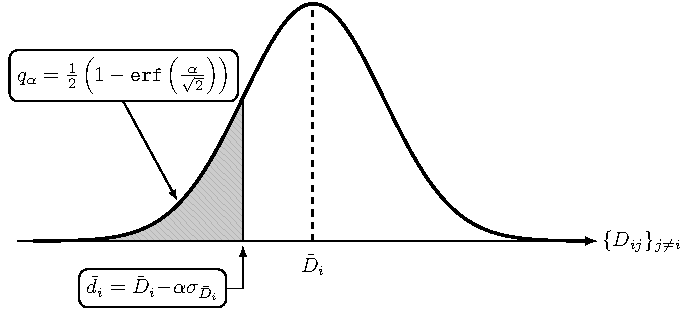
\includegraphics[width=0.95\textwidth]{shaded_bell_curve.pdf}}
\end{minipage}%\hspace{0.15cm}
\begin{minipage}[h]{0.3\textwidth}
\noindent\refstepcounter{figure}\textbf{Fig \thefigure \label{fig:gaussPlot}.} Illustration of the expected probability of a fixed instance $j$ being in the fixed radius neighborhood of another instance $i$. The fixed radius is parameterized by a fraction $\alpha$ of the standard deviation of all pairwise distances measured from instance $i$ to all possible neighbors.
\end{minipage}
\end{figure} 

\section{Derivation of means and standard deviations for metrics and data distributions}

\subsection{Magnitude Difference Distribution}

Suppose that $X_{ia}, X_{ja} \overset{iid}{\sim} \mathcal{F}_X(\mu_x,\sigma^2_x)$ and define $Z_a \sim \mathcal{F}_Z(\mu_z,\sigma^2_z)$ such that $Z_a = d_{ij}(a) = |X_{ia} - X_{ja}|$, where $a \in \mathcal{A}$ and $|\mathcal{A}| = p$.

\begin{itemize}
\item[(i)] Suppose that $x_{ia} \geq x_{ja}$. Based on the iid assumption for $X_{ia}$ and $X_{ja}$, it follows that the joint density function $g^{(1)}$ of $X_{ia}$ and $Z_a$ is given by

\begin{equation}
\begin{aligned}
g^{(1)}(x_{ia},z_a) &= f_X(x_{ia},x_{ja})\biggl|\frac{\partial x_{ja}}{\partial z_a}\biggr| \\
&= f_X(x_{ia})f_X(x_{ja})|-1| \\
&= f_X(x_{ia})f_X(x_{ia}-z_a), \quad z_a \geq 0
\end{aligned}
\end{equation}

The density function $f^{(1)}_Z$ of $Z_a$ is then defined as

\begin{equation}
f^{(1)}_Z(z_a) = \int_{-\infty}^{\infty} g^{(1)}(x_{ia},z_a)\text{d}x_{ia} = \int_{-\infty}^{\infty} f_X(x_{ia})f_X(x_{ia}-z_a)\text{d}x_{ia}, \quad z_a \geq 0
\end{equation}

\item[(ii)] Suppose that $x_{ia} < x_{ja}$. Based on the iid assumption for $X_{ia}$ and $X_{ja}$, it follows that the joint density function $g^{(2)}$ of $X_{ia}$ and $Z_a$ is given by

\begin{equation}
\begin{aligned}
g^{(2)}(x_{ia},z_a) &= f_X(x_{ia},x_{ja})\biggl|\frac{\partial x_{ja}}{\partial z_a}\biggr| \\
&= f_X(x_{ia})f_X(x_{ja})|1| \\
&= f_X(x_{ia})f_X(x_{ia}+z_a), \quad z_a \geq 0
\end{aligned}
\end{equation}

The density function $f^{(2)}_Z$ of $Z_a$ is then defined as

\begin{equation}
f^{(2)}_Z(z_a) = \int_{-\infty}^{\infty} g^{(2)}(x_{ia},z_a)\text{d}x_{ia} = \int_{-\infty}^{\infty} f_X(x_{ia})f_X(x_{ia}+z_a)\text{d}x_{ia}, \quad z_a \geq 0
\end{equation}
\end{itemize}

Let $F_Z$ denote the distribution function of the random variable $Z_a$. Furthermore, let $E^{(1)}=\bigl\{X_{ia}-X_{ja} \leq z_a | X_{ia} \geq X_{ja}\bigr\}$ and $E^{(2)}=\bigl\{-X_{ia}+X_{ja} \leq z_a | X_{ia} < X_{ja}\bigr\}$. Then we have

\begin{equation}\label{eq:MagDiffCDF}
\begin{aligned}
F_Z(z_a) &= \text{P}\bigl[Z_a \leq z_a\bigr] \\
&= \text{P}\bigl[|X_{ia} - X_{ja}| \leq z_a\bigr] \\
&= \text{P}\bigl[\bigl\{X_{ia}-X_{ja} \leq z_a | X_{ia} \geq X_{ja}\bigr\} \cup \bigl\{-X_{ia}+X_{ja} \leq z_a | X_{ia} < X_{ja}\bigr\}\bigr] \\
&= \text{P}\bigl[E^{(1)} \cup E^{(2)}\bigr] \\
&= \text{P}\bigl[E^{(1)}\bigr] + \text{P}\bigl[E^{(2)}\bigr] - \text{P}\bigl[E^{(1)} \cap E^{(2)}\bigr] \\
&= \text{P}\bigl[E^{(1)}\bigr] + \text{P}\bigl[E^{(2)}\bigr] \\
&= \int_{-\infty}^{z_a} f^{(1)}_Z(t) \text{d}t + \int_{-\infty}^{z_a} f^{(2)}_Z(t) \text{d}t \\
&= \int_{-\infty}^{z_a} \left(f^{(1)}_Z(t) + f^{(2)}_Z(t)\right) \text{d}t \\
&= \int_{-\infty}^{z_a} \left(\int_{-\infty}^{\infty}f_X(x_{ia})\left[f_X(x_{ia} - t) + f_X(x_{ia} + t)\right] \text{d}x_{ia}\right)\text{d}t, \quad z_a \geq 0
\end{aligned}
\end{equation}

It follows directly from the result in Eq. \ref{eq:MagDiffCDF} that the density function of the random variable $Z_a$ is given by

\begin{equation}\label{eq:MagDiffPDF}
f_Z(z_a) = \frac{\partial}{\partial z_a} F_Z(z_a) = \int_{-\infty}^{\infty} f_X(x_{ia}) \left[f_X(x_{ia} - z_a) + f_X(x_{ia} + z_a)\right] \text{d}x_{ia}, \quad z_a \geq 0
\end{equation}

Using Eq. \ref{eq:MagDiffPDF}, we can compute the mean and variance of the magnitude difference as

\begin{equation}\label{eq:1DMagDiffMean}
\mu_z = \int_{-\infty}^{\infty} z_a f_Z(z_a) \text{d}z_a
\end{equation}

and 

\begin{equation}\label{eq:1DMagDiffVar}
\sigma^2_{z} = \int_{-\infty}^{\infty} z^2_a f_Z(z_a) \text{d}z_a - \mu^2_z.
\end{equation}

It follows immediately from Eqs. \ref{eq:1DMagDiffMean} and \ref{eq:1DMagDiffVar} and the Classical Central Limit Theorem (CCLT) that

\begin{equation}\label{eq:manhattanDistr}
D^{(1)}_{ij} = \sum_{a \in \mathcal{A}} Z_a = \sum_{a \in \mathcal{A}} |X_{ia} - X_{ja}| \overset{.}{\sim} \mathcal{N}\left(\mu_zp,\sigma^2_zp\right)
\end{equation}

\subsubsection{Standard normal data}

If $X_{ia},X_{ja} \overset{iid}{\sim} \mathcal{N}(0,1)$, then the marginal density functions with respect to $X$ for $X_{ia}$, $X_{ia} - Z_a$, and $X_{ia} + Z_a$ are defined as

\begin{equation}\label{eq:normalManXmarg}
f_X(x_{ia}) = \frac{1}{\sqrt{2\pi}}e^{-\frac{1}{2}x^2_{ia}},
\end{equation}

\begin{equation}\label{eq:normalManXMinusZmarg}
f_X(x_{ia} - z_a) = \frac{1}{\sqrt{2\pi}}e^{-\frac{1}{2}(x_{ia} - z_a)^2}, \quad z_a \geq 0, \text{ and}
\end{equation}

\begin{equation}\label{eq:normalManXPlusZmarg}
f_X(x_{ia} + z_a) = \frac{1}{\sqrt{2\pi}}e^{-\frac{1}{2}(x_{ia} + z_a)^2}, \quad z_a \geq 0.
\end{equation}

Substituting the results given by Eqs. \ref{eq:normalManXmarg}-\ref{eq:normalManXPlusZmarg} into Eq. \ref{eq:MagDiffPDF} and completing the square on $x_{ia}$ in the exponents, we have

\begin{equation}\label{eq:normalManPDF}
\begin{aligned}
f_Z(z_a) &= \frac{1}{2\pi}e^{-\frac{1}{4}z^2_a}\int_{-\infty}^{\infty}\left(e^{-\frac{1}{2}\left[\sqrt{2}\left(x_{ia} - \frac{1}{2}z_a\right)\right]^2} + e^{-\frac{1}{2}\left[\sqrt{2}\left(x_{ia} + \frac{1}{2}z_a\right)\right]^2}\right)\text{d}x_{ia}, \quad z_a \geq 0\\
&= \frac{1}{2\sqrt{\pi}}e^{-\frac{1}{4}z^2_a}\int_{-\infty}^{\infty}\frac{1}{\sqrt{2\pi}}\left(e^{-\frac{1}{2}u^2} + e^{-\frac{1}{2}u^2}\right)\text{d}u, \quad z_a \geq 0\\
&= \frac{1}{2\sqrt{\pi}}e^{-\frac{1}{4}z^2_a}(1 + 1), \quad z_a \geq 0\\
&= \frac{1}{2\sqrt{\pi}}e^{-\frac{1}{4}z^2_a} + \frac{1}{2\sqrt{\pi}}e^{-\frac{1}{4}z^2_a}, \quad z_a \geq 0 \\
&= \frac{1}{\sqrt{\pi}}e^{-\frac{1}{2}\left(\frac{z_a}{\sqrt{2}}\right)^2}, \quad z_a \geq 0 \\
&= \frac{\sqrt{2}}{\sqrt{2}\sqrt{\pi}} e^{-\frac{1}{2}\left(\frac{z_a}{\sqrt{2}}\right)^2}, \quad z_a \geq 0
\end{aligned}
\end{equation}

The density function given by Eq. \ref{eq:normalManPDF} is a half-normal (or folded normal) density with scale parameter $\sigma = \sqrt{2}$. This distribution has mean and variance given by

\begin{equation}\label{eq:normalAbsDiffMean}
\begin{aligned}
\mu_z &= \frac{\sigma \sqrt{2}}{\sqrt{\pi}} \\
&= \frac{2}{\sqrt{\pi}}
\end{aligned}
\end{equation}

\noindent and

\begin{equation}\label{eq:normalAbsDiffVar}
\begin{aligned}
\sigma^2_z &= \sigma^2\left(1 - \frac{2}{\pi}\right) \\
&= \frac{2(\pi-2)}{\pi}.
\end{aligned}
\end{equation}

By linearity of the expected value and variance operators under the iid assumption, Eqs. \ref{eq:normalAbsDiffMean} and \ref{eq:normalAbsDiffVar} allow the $p\text{-dimensional}$ mean and variance of the $D^{(1)}_{ij}$ distribution to be computed directly as

\begin{equation}\label{eq:normalManMean}
\mu_{D^{(1)}_{ij}} = \text{E}\left(D^{(1)}_{ij}\right) = \text{E}\left(\sum_{a \in \mathcal{A}} Z_a\right) = \sum_{a \in \mathcal{A}} \text{E}\left(Z_a\right) = \sum_{a \in \mathcal{A}} \frac{2}{\sqrt{\pi}} = \frac{2p}{\sqrt{\pi}}
\end{equation}

\noindent and

\begin{equation}\label{eq:normalManVar}
\sigma^2_{D^{(1)}_{ij}} = \text{Var}\left(D^{(1)}_{ij}\right) = \text{Var}\left(\sum_{a \in \mathcal{A}} Z_a\right) = \sum_{a \in \mathcal{A}} \text{Var}\left(Z_a\right) = \sum_{a \in \mathcal{A}} \frac{2(\pi - 2)}{\pi} = \frac{2(\pi - 2)p}{\pi}
\end{equation}

Therefore, the asymptotic distribution of $D^{(1)}_{ij}$ for standard normal data is

\begin{equation}\label{eq:normalManDistr}
\mathcal{N}\left(\frac{2p}{\sqrt{\pi}},\frac{2(\pi - 2)p}{\sqrt{\pi}}\right)
\end{equation}

\subsubsection{Standard uniform data}

If $X_{ia},X_{ja} \overset{iid}{\sim} \mathcal{U}(0,1)$, then the marginal density functions with respect to $X$ for $X_{ia}$, $X_{ia} - Z_a$, and $X_{ia} + Z_a$ are defined as

\begin{equation}\label{eq:uniformManXmarg}
f_X(x_{ia}) = 1, \quad 0 \leq x_{ia} \leq 1
\end{equation}

\begin{equation}\label{eq:uniformManXMinusZmarg}
f_X(x_{ia} - z_a) = 1, \quad 0 \leq x_{ia} - z_a \leq 1, \text{ and}
\end{equation}

\begin{equation}\label{eq:uniformManXPlusZmarg}
f_X(x_{ia} + z_a) = 1, \quad 0 \leq x_{ia} + z_a \leq 1.
\end{equation}

Substituting the results given by Eqs. \ref{eq:uniformManXmarg}-\ref{eq:uniformManXPlusZmarg}, we have

\begin{equation}\label{eq:uniformManPDF}
\begin{aligned}
f_Z(z_a) &= \int_{-\infty}^{\infty}f_X(x_{ia})[f_X(x_{ia} - z_a) + f_X(x_{ia} + z_a)]\text{d}x_{ia}, \quad z_a \geq 0 \\
&= \int_{0}^{1}[f_X(x_{ia} - z_a) + f_X(x_{ia} + z_a)]\text{d}x_{ia}, \quad z_a \geq 0 \\
&= \int_{z_a}^{1}1\text{d}x_{ia} + \int_{0}^{1 - z_a}1\text{d}x_{ia}, \quad z_a \geq 0 \\
&= (1 - z_a) + (1 - z_a), \quad z_a \geq 0 \\
&= 2(1 - z_a), \quad z_a \geq 0
\end{aligned}
\end{equation}

The density given by Eq. \ref{eq:uniformManPDF} is a triangular density 

\begin{equation}\label{eq:triangle}
f_Z(z_a) = \frac{2(b - z_a)}{(b - a)(b - c)}, \quad c \leq z_a \leq b 
\end{equation}

\noindent with parameters $a = 0$, $b = 1$, and $c = 0$ with mean and variance given by

\begin{equation}\label{eq:uniformAbsDiffMean}
\begin{aligned}
\mu_z &= \frac{a + b + c}{3} \\
&= \frac{1}{3}
\end{aligned}
\end{equation}

\noindent and

\begin{equation}\label{eq:uniformAbsDiffVar}
\begin{aligned}
\sigma^2_z &= \frac{a^2 + b^2 + c^2 - ab - ac - bc}{18} \\
&= \frac{1}{18}
\end{aligned}
\end{equation}

By linearity of the expected value and variance operators under the iid assumption, Eqs. \ref{eq:uniformAbsDiffMean} and \ref{eq:uniformAbsDiffVar} allow the $p \text{-dimensional}$ mean and variance of the $D^{(1)}_{ij}$ distribution to be computed directly as

\begin{equation}\label{eq:uniformManMean}
\mu_{D^{(1)}_{ij}} = \text{E}\left(D^{(1)}_{ij}\right) = \text{E}\left(\sum_{a \in \mathcal{A}}Z_a\right) = \sum_{a \in \mathcal{A}} \text{E}(Z_a) = \sum_{a \in \mathcal{A}}\frac{1}{3} = \frac{p}{3}
\end{equation}

\noindent and

\begin{equation}\label{eq:uniformManVar}
\sigma^2_{D^{(1)}_{ij}} = \text{Var}\left(D^{(1)}_{ij}\right) = \text{Var}\left(\sum_{a \in \mathcal{A}} Z_a\right) = \sum_{a \in \mathcal{A}} \text{Var}\left(Z_a\right) = \sum_{a \in \mathcal{A}} \frac{1}{18} = \frac{p}{18}
\end{equation}

Therefore, the asymptotic distribution of $D^{(1)}_{ij}$ for standard uniform data is

\begin{equation}\label{eq:uniformManDistr}
\mathcal{N}\left(\frac{p}{3},\frac{p}{18}\right)
\end{equation}

\subsection{Squared difference distribution}

Suppose that $X_{ia}, X_{ja} \overset{iid}{\sim} \mathcal{F}_X(\mu_x,\sigma^2_x)$ and define $Z^2_a \sim \mathcal{F}_{Z^2}(\mu_{z^2},\sigma^2_{z^2})$ such that $Z^2_a = d^2_{ij}(a) = (X_{ia} - X_{ja})^2$, where $a \in \mathcal{A}$ and $|\mathcal{A}| = p$.

\begin{itemize}
\item[(i)] Suppose that $x_{ja} = x_{ia} - \sqrt{z^2_a}$. Based on the iid assumption for $X_{ia}$ and $X_{ja}$, it follows that the joint density function $g^{(1)}$ of $X_{ia}$ and $Z^2_a$ is given by

\begin{equation}
\begin{aligned}
g^{(1)}(x_{ia},z^2_a) &= f_X(x_{ia},x_{ja})\biggl|\frac{\partial x_{ja}}{\partial z^2_a}\biggr| \\
&= f_X(x_{ia})f_X(x_{ja})\biggl|\frac{-1}{2\sqrt{z^2_a}}\biggr| \\
&= \frac{1}{2\sqrt{z^2_a}}f_X(x_{ia})f_X(x_{ia}-\sqrt{z^2_a})
\end{aligned}
\end{equation}

The density function $f^{(1)}_{Z^2}$ of $Z^2_a$ is then defined as

\begin{equation}
f^{(1)}_{Z^2}(z^2_a) = \int_{-\infty}^{\infty} g^{(1)}(x_{ia},z^2_a)\text{d}x_{ia} = \int_{-\infty}^{\infty} f_X(x_{ia})f_X(x_{ia}-\sqrt{z^2_a})\text{d}x_{ia}
\end{equation}

\item[(ii)] Suppose that $x_{ja} = x_{ia} + \sqrt{z^2_a}$. Based on the iid assumption for $X_{ia}$ and $X_{ja}$, it follows that the joint density function $g^{(2)}$ of $X_{ia}$ and $Z^2_a$ is given by

\begin{equation}
\begin{aligned}
g^{(2)}(x_{ia},z^2_a) &= f_X(x_{ia},x_{ja})\biggl|\frac{\partial x_{ja}}{\partial z^2_a}\biggr| \\
&= f_X(x_{ia})f_X(x_{ja})\biggl|\frac{1}{2\sqrt{z^2_a}}\biggr| \\
&= \frac{1}{2\sqrt{z^2_a}}f_X(x_{ia})f_X(x_{ia}+\sqrt{z^2_a})
\end{aligned}
\end{equation}

The density function $f^{(2)}_{Z^2}$ of $Z^2_a$ is then defined as

\begin{equation}
f^{(2)}_{Z^2}(z_a) = \int_{-\infty}^{\infty} g^{(2)}(x_{ia},z^2_a)\text{d}x_{ia} = \int_{-\infty}^{\infty} f_X(x_{ia})f_X(x_{ia}+\sqrt{z^2_a})\text{d}x_{ia}
\end{equation}
\end{itemize}

Let $F_Z$ denote the distribution function of the random variable $Z_a$. Furthermore, let $E^{(1)}=\bigl\{(X_{ia}-X_{ja})^2 \leq z^2_a | X_{ja}=X_{ia}-\sqrt{Z^2_a}\bigr\}$ and $E^{(2)}=\bigl\{(X_{ia} - X_{ja})^2 \leq z_a | X_{ja}=X_{ia} + \sqrt{Z^2_a}\bigr\}$. Then we have

\begin{equation}\label{eq:SquDiffCDF}
\begin{aligned}
F_{Z^2}(z^2_a) &= \text{P}\bigl[Z^2_a \leq z^2_a\bigr] \\
&= \text{P}\bigl[(X_{ia} - X_{ja})^2 \leq z^2_a\bigr] \\
&= \text{P}\bigl[\bigl\{(X_{ia}-X_{ja})^2 \leq z^2_a | X_{ja}=X_{ia}-\sqrt{Z^2_a}\bigr\} \cup \\
&\hphantom{=} \quad \quad \bigl\{(X_{ia} - X_{ja})^2 \leq z_a | X_{ja}=X_{ia} + \sqrt{Z^2_a}\bigr\}\bigr] \\
&= \text{P}\bigl[E^{(1)} \cup E^{(2)}\bigr] \\
&= \text{P}\bigl[E^{(1)}\bigr] + \text{P}\bigl[E^{(2)}\bigr] - \text{P}\bigl[E^{(1)} \cap E^{(2)}\bigr] \\
&= \text{P}\bigl[E^{(1)}\bigr] + \text{P}\bigl[E^{(2)}\bigr] \\
&= \int_{-\infty}^{z^2_a} f^{(1)}_{Z^2}(t) \text{d}t + \int_{-\infty}^{z^2_a} f^{(2)}_{Z^2}(t) \text{d}t \\
&= \int_{-\infty}^{z^2_a} \left(f^{(1)}_{Z^2}(t) + f^{(2)}_{Z^2}(t)\right) \text{d}t \\
&= \frac{1}{2\sqrt{z^2_a}}\int_{-\infty}^{z^2_a} \left(\int_{-\infty}^{\infty}f_X(x_{ia})\left[f_X(x_{ia} - t) + f_X(x_{ia} + t)\right] \text{d}x_{ia}\right)\text{d}t, \quad z_a > 0
\end{aligned}
\end{equation}

It follows directly from the result in Eq. \ref{eq:SquDiffCDF} that the density function of the random variable $Z^2_a$ is given by

\begin{equation}\label{eq:SquDiffPDF}
f_{Z^2}(z^2_a) = \frac{\partial}{\partial z^2_a} F_{Z^2}(z^2_a) = \frac{1}{2\sqrt{z^2_a}}\int_{-\infty}^{\infty} f_X(x_{ia}) \left[f_X(x_{ia} - \sqrt{z^2_a}) + f_X(x_{ia} + \sqrt{z^2_a})\right] \text{d}x_{ia}
\end{equation}

Using Eq. \ref{eq:SquDiffPDF}, we can compute the mean and variance of the squared difference as

\begin{equation}\label{eq:1DSquDiffMean}
\mu_{z^2} = \int_{-\infty}^{\infty} z^2_a f_{Z^2}(z^2_a) \text{d}z^2_a
\end{equation}

and

\begin{equation}\label{eq:1DSquDiffVar}
\sigma^2_{z^2} = \int_{-\infty}^{\infty} (z^2_a)^2 f_{Z^2}(z^2_a) \text{d}z^2_a - \mu^2_{z^2}
\end{equation}

It follows immediately from Eqs. \ref{eq:1DSquDiffMean} and \ref{eq:1DSquDiffVar} and the Classical Central Limit Theorem that

\begin{equation}\label{eq:SquDiffDistrGeneral}
\left(D^{(2)}_{ij}\right)^2 = \sum_{a \in \mathcal{A}} Z^2_a = \sum_{a \in \mathcal{A}} (X_{ia} - X_{ja})^2 \overset{.}{\sim} \mathcal{N}\left(\mu_{z^2}p,\sigma^2_{z^2}p\right)
\end{equation}

Then the Delta Method \cite{allStats} can be used to show that

\begin{equation}\label{eq:euclideanDistr}
D^{(2)}_{ij} = \left(\sum_{a \in \mathcal{A}} Z^2_a\right)^{1/2} = \left(\sum_{a \in \mathcal{A}} (X_{ia} - X_{ja})^2\right)^{1/2} \overset{.}{\sim} \mathcal{N}\left(\sqrt{\mu_{z^2}p},\frac{\sigma^2_{z^2}}{4\mu_{z^2}}\right)
\end{equation}

Given that $\text{E}\left[\left(\left[D^{(2)}_{ij}\right]^2\right)^{1/2}\right] = \left(\text{E}\left[\left(D^{(2)}_{ij}\right)^2\right] - \text{Var}\left[\left(\left[D^{(2)}_{ij}\right]^2\right)^{1/2}\right]\right)^{1/2}$, and the results given in Eq. \ref{eq:euclideanDistr} provide an estimate of both $\text{E}\left[\left(D^{(2)}_{ij}\right)^2\right]$ and $\text{Var}\left[\left(\left[D^{(2)}_{ij}\right]^2\right)^{1/2}\right]$, an improved estimate of the mean is given by

\begin{equation}\label{eq:euclideanMean}
\text{E}\left(D^{(2)}_{ij}\right) = \sqrt{\mu_{z^2}p - \frac{\sigma^2_{z^2}}{4\mu_{z^2}}}.
\end{equation}

The asymptotic distribution of $D^{(2)}_{ij}$ with improved estimate of the mean is then given by

\begin{equation}
\mathcal{N}\left(\sqrt{\mu_{z^2}p - \frac{\sigma^2_{z^2}}{4\mu_{z^2}}},\frac{\sigma^2_{z^2}}{4\mu_{z^2}}\right).
\end{equation}

Without loss of generality, the argument leading to and resulting in Eq. \ref{eq:euclideanDistr} can be generalized to the case of $q>2$. This implies that we have the asymptotic distribution of $D^{(q)}$ for all $q \in \mathbb{Z}$.

\subsubsection{Standard normal data}

If $X_{ia},X_{ja} \overset{iid}{\sim} \mathcal{N}(0,1)$, then the marginal density functions with respect to $X$ for $X_{ia}$, $X_{ia} - \sqrt{Z^2_a}$, and $X_{ia} + \sqrt{Z^2_a}$ are defined as

\begin{equation}\label{eq:normalSquDiffXmarg}
f_X(x_{ia}) = \frac{1}{\sqrt{2\pi}} e^{-\frac{1}{2}x^2_{ia}},
\end{equation}

\begin{equation}\label{eq:normalSquDiffXMinusZmarg}
f_X(x_{ia} - z_a) = \frac{1}{\sqrt{2\pi}} e^{-\frac{1}{2}\left(x_{ia} - \sqrt{z^2_a}\right)^2}, \quad z_a \geq 0, \text{ and}
\end{equation}

\begin{equation}\label{eq:normalSquDiffXPlusZmarg}
f_X(x_{ia} + z_a) = \frac{1}{\sqrt{2\pi}} e^{-\frac{1}{2}\left(x_{ia} + \sqrt{z^2_a}\right)^2}, \quad z_a \geq 0.
\end{equation}

Substituting the results given by Eqs. \ref{eq:normalSquDiffXmarg}-\ref{eq:normalSquDiffXPlusZmarg} into Eq. \ref{eq:SquDiffPDF} and completing the square on $x_{ia}$ in the exponents, we have

\begin{equation}\label{eq:normalSquDiffPDF}
\begin{aligned}
f_{Z^2}(z^2_a) &= \frac{1}{4\pi\sqrt{z^2_a}} e^{-\frac{1}{4}z^2_a} \int_{-\infty}^{\infty} \left(e^{-\frac{1}{2}\left(\sqrt{2}x_{ia} - \frac{\sqrt{2}}{2}\sqrt{z^2_a}\right)^2} + e^{-\frac{1}{2}\left(\sqrt{2}x_{ia} + \frac{\sqrt{2}}{2}\sqrt{z^2_a}\right)^2} \right) \text{d}x_{ia}, \\
&\hphantom{= } \hspace{10.8cm} z_a > 0 \\
&= \frac{1}{4\sqrt{\pi z^2_a}} e^{-\frac{1}{4}z^2_a}\int_{-\infty}^{\infty} \frac{1}{\sqrt{2\pi}} \left(e^{-\frac{1}{2}u^2} + e^{-\frac{1}{2}u^2}\right) \text{d}u, \quad z_a > 0 \\
&= \frac{1}{4\sqrt{\pi z^2_a}}e^{-\frac{1}{4}z^2_a}(1 + 1), \quad z_a > 0 \\
&= \frac{1}{2\sqrt{\pi z^2_a}}e^{-\frac{1}{4}z^2_a}, \quad z_a > 0 \\
&= \frac{1}{\sqrt{pi} 4^{1/2}} \left(z^2_a\right)^{-1/2} e^{-\frac{1}{4}z^2_a}, \quad z_a > 0 \\
&= \frac{1}{\Gamma\left(\frac{1}{2}\right) 4^{-1/2}} \left(z^2_a\right)^{\frac{1}{2} - 1} e^{-\frac{1}{4}z^2_a}, \quad z_a > 0
\end{aligned}
\end{equation}

The density function given by Eq. \ref{eq:normalSquDiffPDF} is a Gamma density with shape and scale parameters $\alpha = \frac{1}{2}$ and $\beta = 4$, respectively. This distribution has mean and variance given by

\begin{equation}\label{eq:1DnormalSquDiffMean}
\begin{aligned}
\mu_{z^2} &= \alpha \beta \\
&= 2
\end{aligned}
\end{equation}

\noindent and

\begin{equation}\label{eq:1DnormalSquDiffVar}
\begin{aligned}
\sigma^2_{z^2} &= \alpha \beta^2 \\
&= 8
\end{aligned}
\end{equation}

By linearity of the expected value and variance operators under the iid assumption, Eqs. \ref{eq:1DnormalSquDiffMean} and \ref{eq:1DnormalSquDiffVar} allow the $p \text{-dimensional}$ mean and variance of the $\left(D^{(2)}_{ij}\right)^2$ distribution to be computed directly as

\begin{equation}\label{eq:normalSquDiffMean}
\mu_{\left(D^{(2)}_{ij}\right)^2} = \text{E}\left[\left(D^{(2)}_{ij}\right)^2\right] = \text{E}\left(\sum_{a \in \mathcal{A}} Z^2_a\right) = \sum_{a \in \mathcal{A}} \text{E}\left(Z^2_a\right) = \sum_{a \in \mathcal{A}} 2 = 2p
\end{equation}

\noindent and

\begin{equation}\label{eq:normalSquDiffVar}
\sigma^2_{\left(D^{(2)}_{ij}\right)^2} = \text{Var}\left[\left(D^{(2)}_{ij}\right)^2\right] = \text{Var}\left(\sum_{a \in \mathcal{A}} Z^2_a\right) = \sum_{a \in \mathcal{A}} \text{Var}\left(Z^2_a\right) = \sum_{a \in \mathcal{A}} 8 = 8p
\end{equation}

Therefore, the asymptotic distribution of $\left(D^{(2)}_{ij}\right)^2$ for standard normal data is

\begin{equation}\label{eq:SquDiffDistr}
\mathcal{N}(2p,8p)
\end{equation}

The random variable $D^{(2)}_{ij}$ is just the square root of the squared difference random variable $\left(D^{(2)}_{ij}\right)^2$. Given that this is a smooth function that is continuously differentiable at $\mu_{\left(D^{(2)}_{ij}\right)^2}$, we can use the Delta Method \cite{allStats} to show that

\begin{equation}\label{eq:normalEucDistr}
D^{(2)}_{ij} = \left(\left[D^{(2)}_{ij}\right]^2\right)^{1/2} \overset{.}{\sim} \mathcal{N}\left(\sqrt{2p},\frac{8p}{4 \cdot 2p}\right) = \mathcal{N}(\sqrt{2p},1)
\end{equation}

Using the improved estimate of the mean given by Eq. \ref{eq:euclideanMean}, the asymptotic distribution of $D^{(2)}_{ij}$ is then given by

\begin{equation}\label{eq:normalEucDistr2}
D^{(2)}_{ij} = \left(\left[D^{(2)}_{ij}\right]^2\right)^{1/2} \overset{.}{\sim} \mathcal{N}\left(\sqrt{2p},\frac{8p}{4 \cdot 2p}\right) = \mathcal{N}(\sqrt{2p - 1},1)
\end{equation}

\begin{table}[H]
\caption{Summary of asymptotic distance distributions for common data types. Metrics with subscripts M and E represent Manhattan and Euclidean, respectively. Metrics with superscript $^*$ represent a deviation from the standard metric by attribute range normalization. The function $\Phi^{-1}(x)$ denotes the standard normal quantile function, where $x \in (0,1)$.}
\label{tab:dist_distr_common}
\centering
% trim=left botm right top
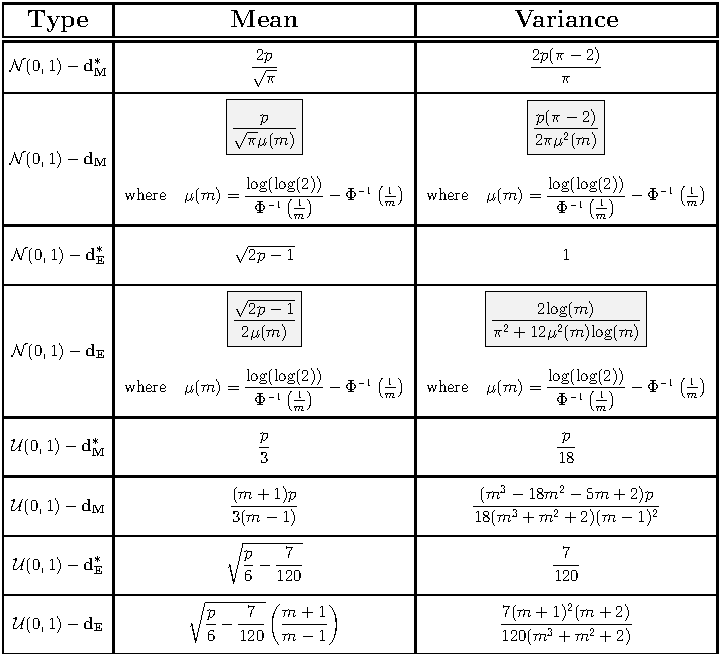
\includegraphics[width=\textwidth]{typical_data-metric_tab.pdf}
\end{table}

\begin{table}[H]
\caption{Summary of asymptotic distance distributions for rs-fMRI and GWAS data. Metrics with superscript $^*$ represent a deviation from the standard metric by attribute range normalization. The function $\Phi^{-1}(x)$ denotes the standard normal quantile function, where $x \in (0,1)$.}
\label{tab:dist_distr_bio}
\centering
% trim=left botm right top
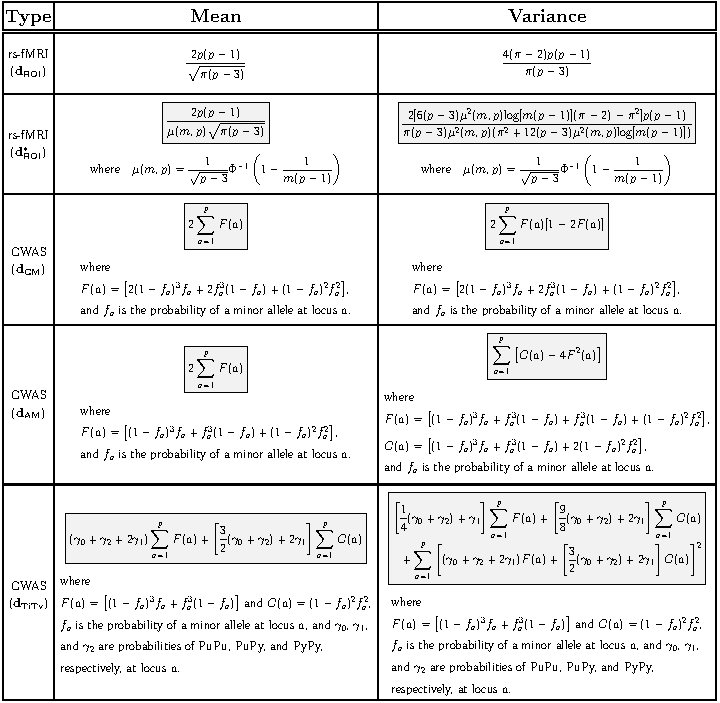
\includegraphics[width=\textwidth]{bioinformaticsy_tab.pdf}
\end{table}

\section{Optimal neighborhood parameters for detecting effects}
k or $\alpha$. 
Balancing blessing and curse of dimensionality.


\section{ICA?}

Using same interaction, increase background noise genes to see degrading of A and B Relief importance because of curse of dimensionality (sparseness).  

\bibliographystyle{unsrt}
\bibliography{BoD}   % name of bib file
\end{document}
